\documentclass[withoutpreface,bwprint]{cumcmthesis}

% Stage 8 论文入口：直接以 LaTeX 组织正文，不经过 Markdown 转换。
\usepackage{amsmath}
\usepackage{amssymb}
\usepackage{booktabs}
\usepackage{tabularx}
\usepackage{graphicx}
\usepackage{longtable}
\usepackage{array}
\usepackage{url}
\usepackage{listings}

\graphicspath{{figures/}}
\setlength{\tabcolsep}{4pt}
\newcommand{\cert}{\text{certified}}
\newcommand{\unres}{\text{unresolved}}
\newcommand{\dd}{\mathrm{d}}

\title{舰船烟幕遮蔽干扰的多阶段证据约束优化模型}
\tihao{B}
\baominghao{000000000000}
\schoolname{匿名参赛学校}
\membera{队员 A}
\memberb{队员 B}
\memberc{队员 C}
\supervisor{指导教师}
\yearinput{2026}
\monthinput{7}
\dayinput{31}

\begin{document}

\maketitle

\begin{abstract}
本文研究来袭威胁与舰船烟幕遮蔽干扰之间的时空耦合决策问题。论文严格沿着“单弹连续优化—单机多弹联合覆盖—多机协同—多威胁因果调度”的主线组织，先用四种连续优化算法生成候选，再用独立的连续覆盖验证器对候选进行认证；随后把起爆事件离散化为有限候选集，并使用局部 SLSQP 精修，最后用保守的时间单元分类给出联合覆盖证书。多机阶段固定为三架 UAV、每架一枚弹，并对航迹半径和成对冲突进行独立检查；多威胁阶段只在已认证任务包上比较因果 rolling、因果 greedy 与离线 hindsight 上界。

在固定的 4\(\times\)4 正式场景矩阵上，Q1 的四算法基准均得到“认证不可行”状态；SHGO 的平均最大连续暴露时长为约 $6.95\,\mathrm{s}$，在本次有限预算基准中最小。Q2 的四个代表场景联合覆盖下界为 $17.2634$--$17.2710\,\mathrm{s}$，相对最佳单烟幕基线的联合增益为 $6.8896$--$6.8971\,\mathrm{s}$；保守验证得到的最大连续暴露下界为 $5.4993$--$6.8956\,\mathrm{s}$。Q3 保持三架 UAV 每架一枚的主解释，路径半径与成对冲突证书均通过，结果与 Q2 的联合覆盖量一致。Q4 在容量 $4$、$2$、$1$ 下三种策略的值分别为 $46.4$、$33.0$、$17.2$，但任务包中仍保留未揭示任务，因此状态标记为未解析。

灵敏度结果表明，在给定的局部扰动范围内，导引响应率的检测时长保持 $24.1677\,\mathrm{s}$，响应延迟从 $1.5$ 增至 $3.0\,\mathrm{s}$ 时可用检测窗口从 $19.1677$ 降至 $17.6677\,\mathrm{s}$，烟幕漂移上界为 $40\,\mathrm{m}$ 时最小间隙约为 $0.0014\,\mathrm{m}$。本文强调这些结果是固定场景、有限候选、证书约束下的可复核结果，不宣称完整 SIP、完整 Pareto 求解、滚动 MILP 或连续全局最优。

\keywords{烟幕遮蔽\quad 连续覆盖认证\quad 事件候选\quad 多机协同\quad 因果调度}
\end{abstract}

% 电子版按要求不生成目录、图目录或表目录；摘要是第一页。
\section{问题重述}

\subsection{研究背景}

舰船在复杂海空威胁环境中需要在有限的反应时间内完成侦测、释放和机动。烟幕弹的效果并不是一个静态几何覆盖问题：目标与来袭威胁都在运动，烟幕云团随时间膨胀、保持和衰减，释放平台还受到航迹长度、反应延迟和作用半径的限制。因此，一个仅在单个时刻判断“是否遮蔽”的模型，不能直接回答连续时间内的遮蔽持续性和最坏暴露问题。

本文将题目中的决策链拆解为四个层次。第一层研究单枚烟幕弹的连续起爆时刻和中心时刻；第二层研究同一架 UAV 携带多枚烟幕弹时的事件组合与联合覆盖；第三层研究多架 UAV 分担烟幕弹后的航迹可行性和协同覆盖；第四层把前述已认证任务包交给一个带有揭示时刻的多威胁调度器。

\subsection{四个子问题}

\begin{enumerate}
  \item \textbf{单弹连续优化（Q1）}：在给定威胁场景、舰船运动和反应延迟下，寻找释放/起爆相关的连续决策，使遮蔽覆盖更长、最大连续暴露更短，同时保留航迹约束。需要比较四类候选算法，并使用独立验证器复核。
  \item \textbf{单机多弹联合覆盖（Q2）}：同一架 UAV 依次释放至多三枚烟幕弹。需要把事件时刻限制到有限候选集，再进行局部精修，使用保守的连续时间覆盖证书区分已覆盖、已暴露和未解析区间。
  \item \textbf{多机协同（Q3）}：固定三架 UAV，每架恰好一枚烟幕弹。需要检查每架 UAV 的作用半径、任意两架之间的路径冲突，并以带 $\varepsilon$ 阈值的词典序规则选择联合方案。
  \item \textbf{多威胁因果调度（Q4）}：从 Q1--Q3 已认证的任务包出发，在任务揭示过程中比较因果 rolling、因果 greedy 与离线 hindsight 上界；未揭示或未认证的任务不能提前消耗容量。
\end{enumerate}

本文的边界是“可审计的有限搜索与验证”。论文不把有限预算算法的最好候选写成连续全局最优，也不把离线 hindsight 上界写成在线策略；这些限制直接由结果文件的 \texttt{global\_optimum\_claim=false}、Q4 的 \texttt{causal} 字段和独立验证代码体现。

\subsection{研究对象与输出}

研究对象为四个正式场景中的代表性前向威胁矩阵行，以及 Q1 生成的 $4\times4$ 正式矩阵。输出包括候选决策、覆盖下界/上界、总暴露与最大连续暴露、最小安全裕度、航迹距离、路径冲突证书、资源容量下的调度值和局部灵敏度结果。所有论文数值均来自 \path{results/q1_rebuild/}、\path{results/q2_rebuild/}、\path{results/q3_rebuild/}、\path{results/q4_rebuild/} 和 \path{results/sensitivity_rebuild/}，证据等级与允许措辞见论文审计表。

\section{问题分析}

\subsection{从连续决策到事件候选}

Q1 的变量本质上是低维连续变量，起爆时刻与烟幕中心时刻决定了烟幕云团在威胁检测区间内的相对位置。直接把每个时刻都作为优化变量会引入不必要的维数，因此代码把物理事件写入候选构造器，优化器只负责在二维边界内评价有限数量的决策向量。四种算法共享同一个候选评价和同一个独立验证器，比较因此具有可比性。

Q2 继续利用“事件优先”的结构：将检测区间端点、烟幕爆炸/保持/失效时刻和 Q1 暖启动事件放入时间网格，枚举有限的有序组合，之后使用 SLSQP 在事件附近做局部精修。候选不是自动可行的；每一个候选仍需要经过航迹半径认证和联合覆盖认证。覆盖证书对每个时间单元使用膨胀目标与收缩烟幕盘判断覆盖，只有固定见证点在整段时间内保持有效时才把单元记为认证暴露，否则继续二分或保留为未解析。

\subsection{从单机到多机}

Q3 将三架 UAV 的主解释固定为“一架一枚”，避免把“至多一枚”放松问题误写成题目主问题。每架 UAV 的路径由单弹构造器生成，再分别通过作用半径证书；任意两条路径都通过成对分离证书。联合覆盖继续调用 Q2 的保守验证器，最后按认证状态、冲突证书、覆盖下界、最大连续暴露和最小成对距离依次排序。

\subsection{从覆盖到因果资源分配}

Q4 的输入不再是连续轨迹，而是 Q1--Q3 输出的任务包：每个任务有揭示时刻、价值、资源成本、认证覆盖下界和认证标志。rolling 在当前时刻只把已经揭示且认证、并且成本不超过剩余容量的任务放入可选集合；greedy 仅改变选择规则；hindsight 作为离线子集枚举上界，不代表可在线执行的策略。这一层的关键不是宣称一个更强的优化器，而是保持信息因果性，避免未揭示结果泄漏到当前决策中。

\begin{figure}[!htbp]
  \centering
  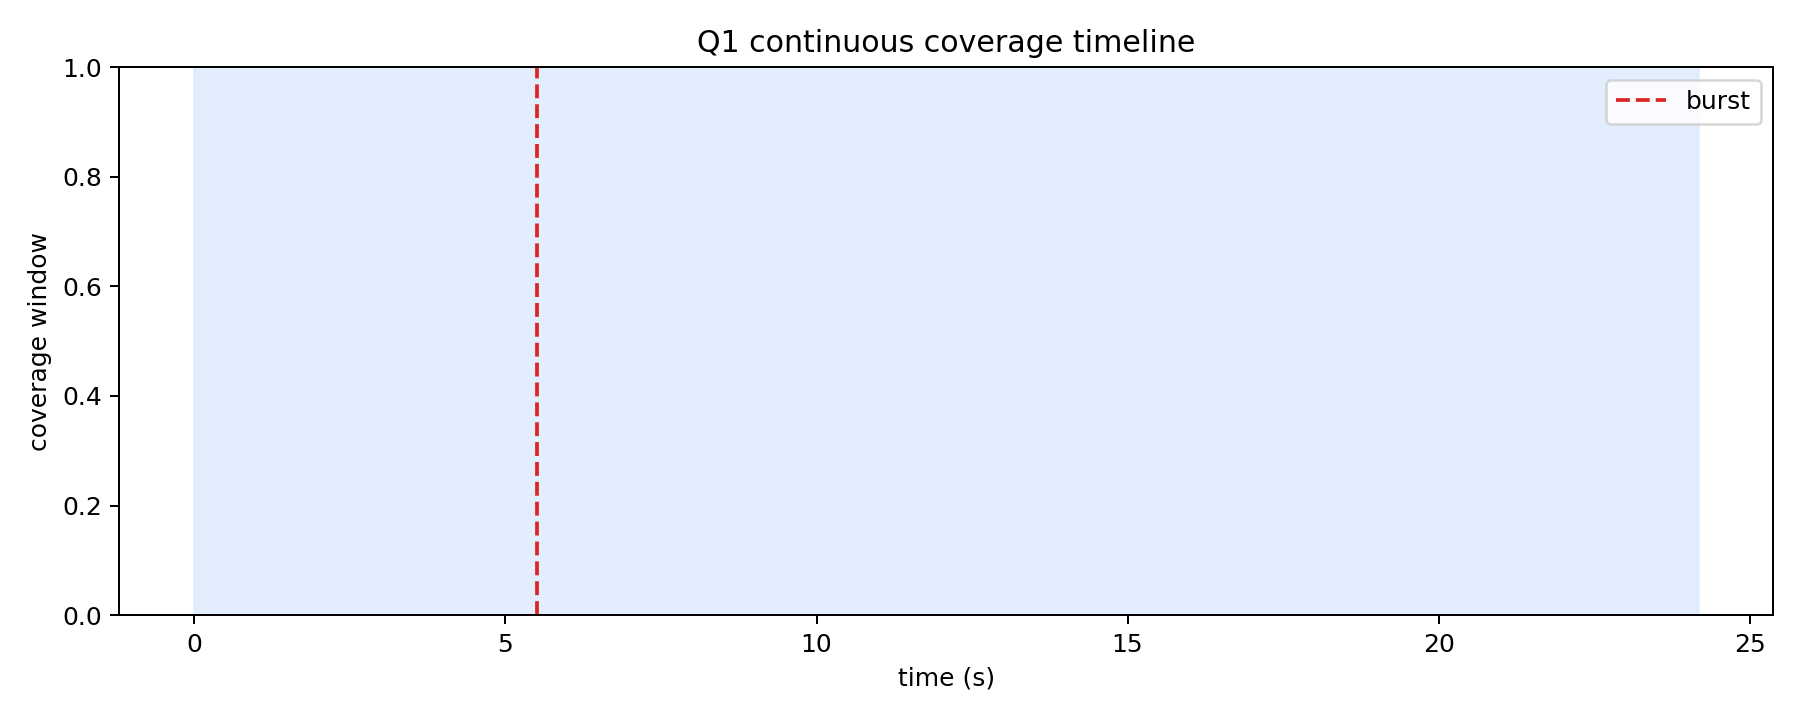
\includegraphics[width=0.88\textwidth]{q1_coverage_timeline.png}
  \caption{冻结基线中的 Q1 连续覆盖时间线（论文仅复用既有图表）。}
  \label{fig:q1-timeline}
\end{figure}

\subsection{验证优先的总流程}

本文采用“候选生成—独立验证—证书分层—词典序筛选—结果审计”的总流程。生成器只提供候选，验证器重新计算路径、烟幕中心和覆盖区间；证书将认证可行、认证不可行和未解析区分开；审计表把正文声明和具体 CSV/JSON/源码行绑定。这样做的目的，是让一项数值声明能够回到可复核的文件和算法，而不是把图表或优化器日志当作充分证明。

\section{模型假设与符号说明}

\subsection{模型假设}

在不改变代码中正式基线定义的前提下，本文采用以下假设：

\begin{enumerate}
  \item 舰船和威胁的运动由场景与常数对象确定，在一次候选评价期间不随机改变；烟幕几何由起爆时刻、中心和半径函数确定。
  \item 正式 Q1--Q3 场景使用 \texttt{formal\_baseline} 模型；丢失导引等情形只作为敏感性文件中明确标记的实验性反事实，不回写正式基线。
  \item UAV 采用代码中的分段线性航迹构造，释放/起爆之间的延迟和同一架 UAV 的释放间隔采用固定约束。
  \item 覆盖认证使用保守的目标外包络和烟幕内包络；无法被整段时间证实的单元保留为未解析，不默认为暴露。
  \item Q4 任务只有在揭示、容量可行且 \texttt{certified=true} 时才可被调度；hindsight 只作为离线上界。
  \item 所有统计量都对应冻结基线、固定随机种子与有限评估预算，论文只报告文件中已有的量，不外推到未计算的场景。
\end{enumerate}

\subsection{符号说明}

\begin{table}[!htbp]
\centering
\caption{主要符号与证据字段}
\label{tab:symbols}
\begin{tabularx}{\textwidth}{>{\centering\arraybackslash}p{0.13\textwidth} X >{\centering\arraybackslash}p{0.18\textwidth}}
\toprule
符号/字段 & 含义 & 单位或取值 \\
\midrule
$t$ & 连续时间变量 & s \\
$t_b$ & 烟幕爆炸时刻 & s \\
$t_c$ & 烟幕中心对应的舰船时刻 & s \\
$t_d$ & UAV 释放时刻 & s \\
$t_0$ & 指令发出时刻 & s \\
$R_s(t)$ & 烟幕在时刻 $t$ 的半径 & m \\
$D(t)$ & 检测区间或检测组件 & s \\
$C(t)$ & 目标舰船覆盖盘 & m \\
$\mathcal{S}$ & 烟幕盘集合 & 集合 \\
$L_{\max}$ & 最大连续暴露时长 & s \\
$G$ & 联合覆盖相对最佳单烟幕的增益 & s \\
$m_{\min}$ & 最小覆盖裕度 & m \\
$d_{\mathrm{flight}}$ & UAV 分段航迹长度 & m \\
$\varepsilon$ & 词典序比较中的数值容差 & 无量纲 \\
\texttt{certified} & 任务/候选是否通过认证 & Boolean \\
\texttt{unresolved} & 仍存在未解析单元或任务 & 状态标记 \\
\texttt{capacity} & Q4 可用资源容量 & 枚/单位 \\
\bottomrule
\end{tabularx}
\end{table}

符号表中的“覆盖”均指验证器给出的覆盖下界或明确标注的区间；没有下标的文字性“覆盖”在结果段落中会同时说明其来源，防止把上界、下界和连续暴露混为一个指标。

\section{统一模型与证据边界}

\subsection{几何覆盖与时间分类}

设舰船在时刻 $t$ 的中心为 $x_T(t)$，有效半径为 $r_T$；第 $j$ 枚烟幕中心和半径分别为 $x_j(t)$、$r_j(t)$。在二维截面中，目标盘可写成
\begin{equation}
  \mathcal{D}_T(t)=\{x:\|x-x_T(t)\|_2\le r_T\},
  \label{eq:target-disk}
\end{equation}
烟幕联合覆盖集合为
\begin{equation}
  \mathcal{D}_S(t)=\bigcup_{j=1}^{k}\{x:\|x-x_j(t)\|_2\le r_j(t)\}.
  \label{eq:smoke-union}
\end{equation}
代码的连续验证器不以单个采样点作为持续覆盖证据，而是对时间单元 $I=[t_l,t_r]$ 使用保守外包络：目标盘半径增加舰船速度上界乘以半单元长度，烟幕盘半径按衰减速度收缩。若外目标盘被内烟幕并集覆盖，则认证整个单元为覆盖；若精确目标盘被认证不可行，且存在一个固定空间见证点在单元内始终位于目标盘内、所有烟幕盘外，则认证为暴露，否则继续细分。

对检测区间进行完整分类，得到
\begin{equation}
  D = D_{\mathrm{cov}}\ \dot\cup\ D_{\mathrm{exp}}\ \dot\cup\ D_{\mathrm{unres}},
  \label{eq:time-partition}
\end{equation}
其中 $D_{\mathrm{unres}}$ 不会被默认为暴露。联合覆盖下界和上界分别由认证覆盖区间和覆盖区间加未解析区间给出；最大连续暴露只对已认证暴露区间取最大长度。

\subsection{延迟与航迹约束}

正式基线中指令、释放和爆炸满足
\begin{align}
  t_d-t_0 &= \tau_{\mathrm{cmd}}, \\
  t_b-t_d &= \tau_{\mathrm{burst}}, \\
  t_0 &\ge 0.
  \label{eq:delays}
\end{align}
候选构造器先生成分段线性 UAV 航迹，再独立重新计算爆炸位置、作用半径和航迹长度。如果候选的路径与烟幕中心不一致，或者超过操作半径，则直接给出认证不可行，而不是由优化器的原生成功标志代替。

\subsection{候选排序}

Q1--Q3 使用成功优先的词典序。以 $s$ 表示认证状态等级，$g$ 表示覆盖下界，$L$ 表示最大连续暴露，$m$ 表示最小裕度，$d$ 表示航迹/资源代价，一个代表性排序向量为
\begin{equation}
  \rho=(s,\ \mathrm{conflict\_ok},\ g,\ -L,\ m,\ -d).
  \label{eq:lexicographic-rank}
\end{equation}
代码在需要时使用显式的 $\varepsilon$ 容差处理数值相等，而不把浮点数近似误解为新的科学结果。因而“benchmark winner”只表示在给定算法、种子、预算和排序规则下的相对结果。

\subsection{证据等级}

本文将证据划分为四级：A 级为 CSV 与 JSON 同时给出并通过 artifact check 的结果；B 级为 JSON 中的结构化算法标志或路径证书；C 级为既有图表对 A/B 级结果的可视化；D 级为代码明确标记的实验性反事实。正文定量结论优先使用 A 级；D 级只用于说明敏感性方向，不用于证明正式方案可行。

\section{Q1：单弹连续优化与独立认证}

\subsection{决策变量与候选构造}

Q1 对每个正式场景使用两个主要连续变量：爆炸时刻 $t_b$ 和烟幕中心对应的舰船时刻 $t_c$。释放时刻和指令时刻由式\eqref{eq:delays}反推，烟幕中心取舰船在 $t_c$ 的位置，UAV 从起飞点到释放点采用分段线性航迹。候选构造器在生成几何对象时已经固定延迟关系，但认证器仍重新检查这些关系。

对候选 $z=(t_b,t_c)$，代码先构造烟幕对象与 UAV 路径，再进行连续覆盖评价。形式化地，可把本阶段的候选目标写成
\begin{equation}
  \max_{z\in\Omega}\quad \left(\,C(z),\ -L(z),\ M(z),\ -F(z)\,\right),
  \label{eq:q1-objective}
\end{equation}
其中 $C$ 是认证覆盖时长，$L$ 是最大连续暴露，$M$ 是最小覆盖裕度，$F$ 是航迹距离；实际选择遵循状态优先的词典序，而不是把这些量任意加权为单一目标。

\subsection{四算法 benchmark}

为避免把某一种优化器的原生返回值当作事实，Q1 对相同场景和固定种子比较四类算法：多起点 SLSQP、Sobol+SLSQP、SHGO、差分进化+SLSQP。每种方法的评估预算为 $24$，候选经过同一独立验证器。Sobol+SLSQP 的局部起点来自同一词典序中最好的有效缓存样本；SHGO 和差分进化仍只是有限预算候选搜索。SLSQP 的序列二次规划背景见文献\cite{kraft1988slsqp,byrd1995sqp}，SHGO 与差分进化分别参考\cite{endes2018shgo,storn1997differential}，这里只复述代码实际调用的有限比较。

四种方法共享变量边界和候选评价器。若 $z^{(r)}$ 是第 $r$ 次评估的向量，则缓存记录为
\begin{equation}
  \mathcal{K}=\{(z^{(r)},\,C^{(r)},\,L^{(r)},\,M^{(r)},\,F^{(r)},\,s^{(r)})\}_{r=1}^{24}.
  \label{eq:q1-cache}
\end{equation}
从缓存中选取暖启动和最终候选都使用同一排序函数
\begin{equation}
  \operatorname{rank}_1(r)=\bigl(s^{(r)},C^{(r)},-L^{(r)},M^{(r)},-F^{(r)},-r\bigr),
  \label{eq:q1-rank}
\end{equation}
最后一项以评估顺序提供确定性平局处理。该设置避免用不同的暖启动准则和最终准则比较两个不同候选。

\begin{table}[!htbp]
\centering
\caption{Q1 四算法基准（4 个前向场景，均为认证不可行）}
\label{tab:q1-benchmark}
\begin{tabular}{lrrrr}
\toprule
方法 & 场景数 & 平均覆盖/s & 平均最大暴露/s & 原生成功次数 \\
\midrule
多起点 SLSQP & 4 & 10.38 & 6.99 & 0 \\
Sobol+SLSQP & 4 & 10.38 & 8.58 & 3 \\
SHGO & 4 & 10.38 & 6.95 & 4 \\
差分进化+SLSQP & 4 & 10.38 & 9.42 & 3 \\
\bottomrule
\end{tabular}
\end{table}

表\ref{tab:q1-benchmark}的平均值由 \path{results/q1_rebuild/q1_algorithm_benchmark.csv} 按方法聚合，原生成功次数不等于认证可行次数。四种方法的验证状态均为 \texttt{certified\_infeasible}，因此 SHGO 的“较小平均最大暴露”只能解释为本次 benchmark 中的相对优胜，不能写成对连续问题的全局证明。

\subsection{独立 verifier 与正式矩阵}

独立验证器依次检查指令/释放延迟、释放位置到爆炸中心的一致性、操作半径、连续覆盖、最大连续暴露和最小裕度。正式 $4\times4$ 场景矩阵共 $16$ 行，CSV 与 JSON 均报告 \texttt{certified\_infeasible}。正式 SHGO 结果的覆盖时长均约为 $10.3761\,\mathrm{s}$；最大连续暴露在 $6.8958$--$7.4931\,\mathrm{s}$ 之间，最小覆盖裕度的最小值为 $-177.7720\,\mathrm{m}$，最大航迹距离为 $529.6218\,\mathrm{m}$。

\begin{table}[!htbp]
\centering
\caption{Q1 正式矩阵按威胁方向的范围核对}
\label{tab:q1-direction}
\begin{tabular}{lrrrr}
\toprule
方向 & 检测时长/s & 覆盖时长/s & 最大连续暴露/s & 最小裕度/m \\
\midrule
front & 24.168 & 10.376 & 6.896--6.903 & $-173.225$--$-173.167$ \\
rear & 25.361 & 10.376 & 7.492--7.493 & $-177.772$--$-177.767$ \\
side & 24.764--24.773 & 10.376 & 7.195--7.212 & $-175.605$--$-175.476$ \\
oblique & 25.186--25.191 & 10.376 & 7.406--7.435 & $-177.109$--$-176.862$ \\
\bottomrule
\end{tabular}
\end{table}

方向范围表直接由 Q1 正式结果 JSON 的 4 个方向分组复算；它只作摘要性核验，具体每一行仍以 \path{results/q1_rebuild/q1_results.csv} 为准。

\begin{figure}[!htbp]
  \centering
  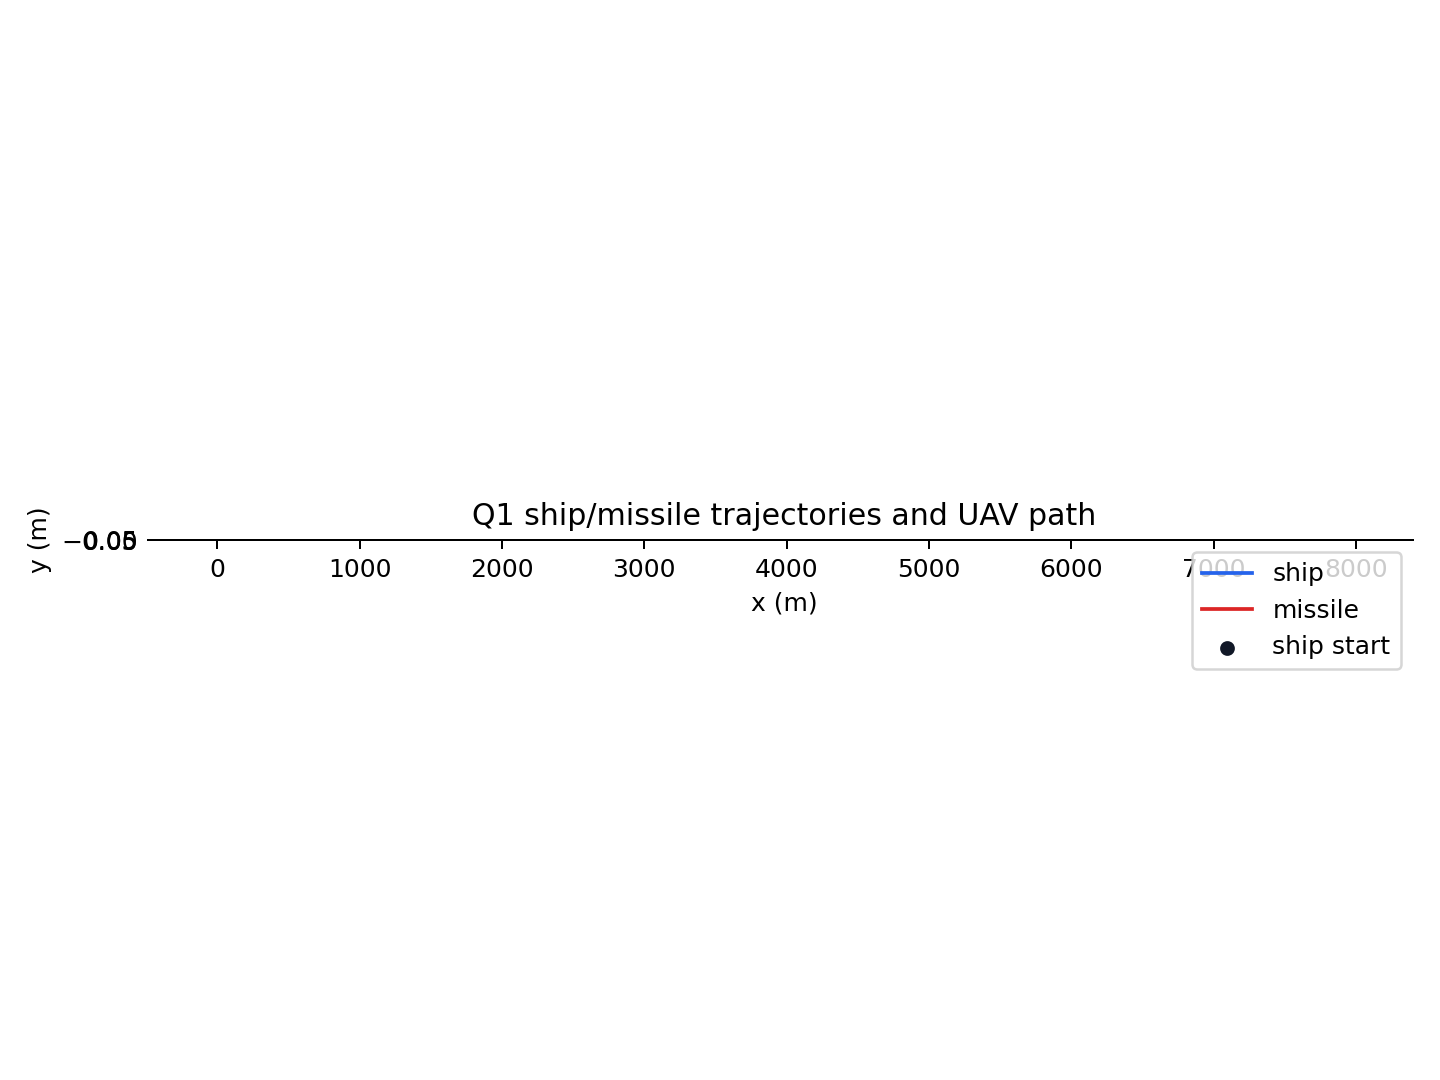
\includegraphics[width=0.82\textwidth]{q1_trajectories.png}
  \caption{Q1 冻结基线的候选航迹。}
  \label{fig:q1-trajectories}
\end{figure}

需要说明的是，冻结的 Q1 时间线图没有绘制绿色覆盖色带；覆盖时长 $10.3761\,\mathrm{s}$ 来自 CSV/JSON 的验证字段，而不是从图中目测得到。论文保留原图以保证图表来源不漂移，数值以结构化结果文件为准。

\begin{figure}[!htbp]
  \centering
  \begin{minipage}[c]{0.48\textwidth}
    \centering
    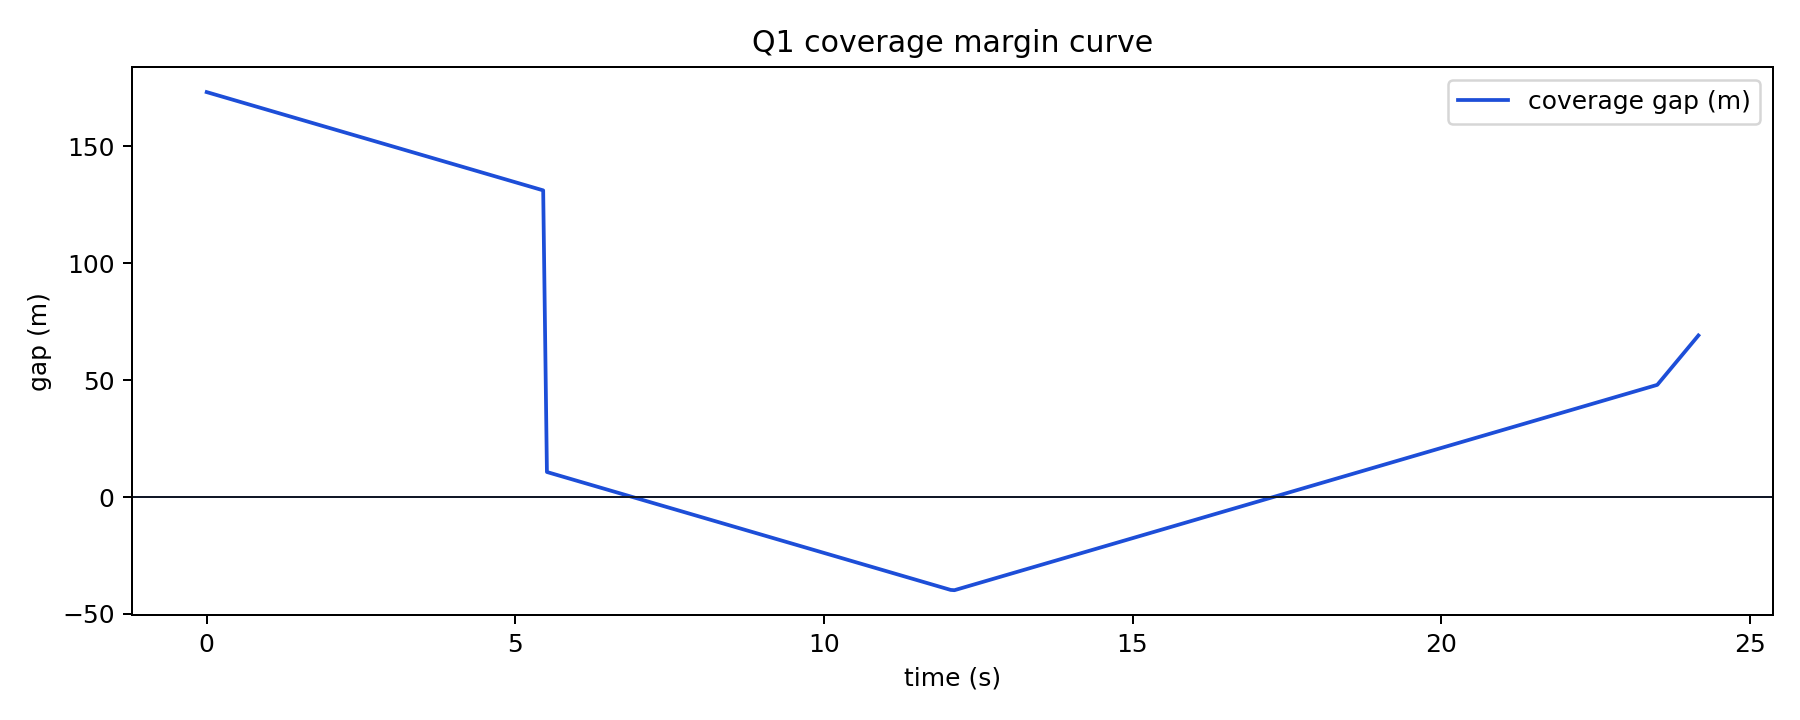
\includegraphics[width=0.96\textwidth]{q1_margin_curve.png}
    \subcaption{覆盖裕度曲线}
  \end{minipage}
  \begin{minipage}[c]{0.48\textwidth}
    \centering
    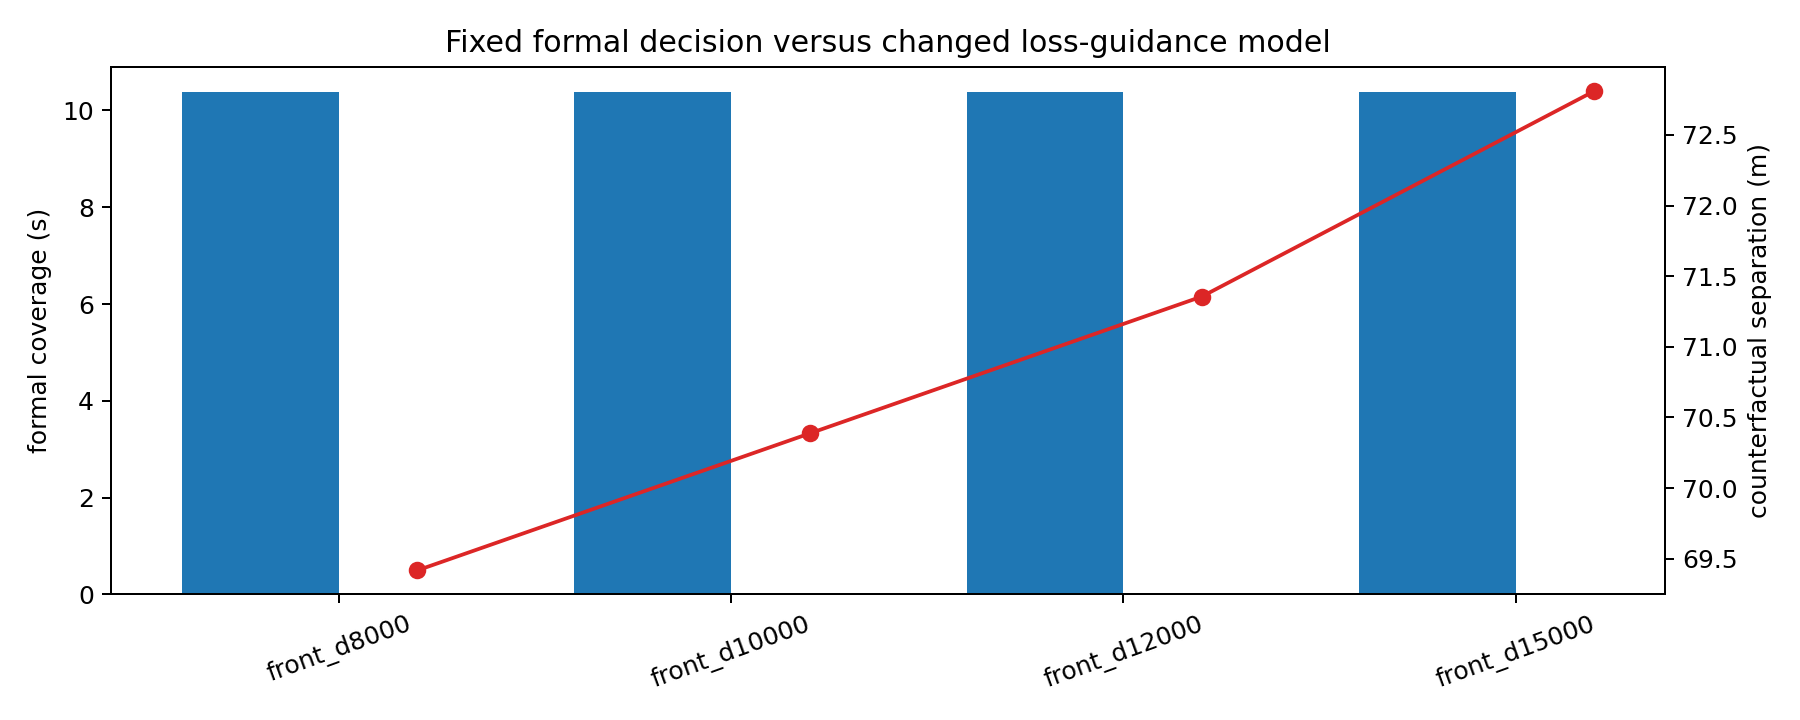
\includegraphics[width=0.96\textwidth]{q1_counterfactual_comparison.png}
    \subcaption{实验性丢失导引反事实}
  \end{minipage}
  \caption{Q1 正式验证与实验性反事实的图表证据。}
  \label{fig:q1-evidence}
\end{figure}

\subsection{反事实边界}

丢失导引图只重建正式候选的决策字段，改变模型层并标记 \texttt{formal\_baseline=false}；它不是 Q1 正式结果，也没有被用于改变四算法 benchmark 的排名。这个边界使“模型敏感性”与“正式认证”保持分离。

\subsection{Q1 小结}

Q1 的可信结论是：四种算法在固定预算下都提供了可复核候选，SHGO 在平均最大连续暴露这一 benchmark 指标上最小；独立 verifier 对正式矩阵全部给出认证不可行。论文不把该结果表述为完整连续全局求解，也不把优化器的 \texttt{native\_success} 直接等同于物理可行。

\section{Q2：单机多弹联合覆盖}

\subsection{有限事件候选}

Q2 将同一架 UAV 的多枚烟幕弹表示为有序爆炸时刻元组
\begin{equation}
  \mathbf{t}_b=(t_{b,1},\ldots,t_{b,k}),\qquad 1\le k\le3,
  \quad t_{b,1}<\cdots<t_{b,k}.
  \label{eq:q2-events}
\end{equation}
候选网格由检测端点、Q1 暖启动事件以及烟幕事件断点组成；代码枚举有限组合并设置最大候选数。对于每个候选，中心时刻由暖启动偏移或爆炸事件计算，路径连接器检查 UAV 在相邻释放事件之间是否可达，并要求同一 UAV 的相邻释放间隔至少为 $1\,\mathrm{s}$。

\subsection{SLSQP 精修}

对有限事件候选，代码把爆炸时刻和中心偏移送入 SLSQP 做局部精修；精修结果仍需重建计划并通过同一验证器。实际返回对象明确写成“best known candidate under a bounded search”，因此该过程不是完整混合整数非线性规划，也不是连续全局最优求解。候选排序使用
\begin{equation}
  \rho_2=(s,\ g,\ -L,\ G,\ -u),
  \label{eq:q2-rank}
\end{equation}
其中 $s$ 为认证状态，$g$ 为联合覆盖下界，$L$ 为最大连续暴露，$G$ 为相对最佳单烟幕基线的联合增益，$u$ 为未解析量或代价字段。

\subsection{保守联合覆盖认证}

对每个检测组件，验证器将烟幕爆炸、保持结束和失效时刻加入断点集合。对每个时间单元，先检验保守覆盖；如果失败，再检验精确目标盘是否认证不可行。只有当精确不可行且固定空间见证点在整个单元内持续位于目标盘内、烟幕盘外时，才把该单元加入认证暴露集合；否则二分，直至达到时间容差并将单元保留为未解析。于是
\begin{equation}
  G=C_{\mathrm{joint,lower}}-C_{\mathrm{single,best,lower}},
  \label{eq:q2-gain}
\end{equation}
而不是把联合覆盖下界本身误叫做 gain。

对一个时间单元 $I$，若保守目标盘为 $\widehat{\mathcal{D}}_T(I)$，收缩后的烟幕盘为 $\check{\mathcal{D}}_S(I)$，则覆盖证书使用充分条件
\begin{equation}
  \widehat{\mathcal{D}}_T(I)\subseteq\check{\mathcal{D}}_S(I)
  \quad\Longrightarrow\quad I\subseteq D_{\mathrm{cov}}.
  \label{eq:q2-covered-cell}
\end{equation}
若一个固定见证点 $w$ 在整个单元内满足
\begin{equation}
  w\in\mathcal{D}_T(t),\qquad
  w\notin\mathcal{D}_{S,j}(t)\quad(j=1,\ldots,k),\qquad \forall t\in I,
  \label{eq:q2-exposed-cell}
\end{equation}
才有 $I\subseteq D_{\mathrm{exp}}$。否则，当 $|I|$ 大于时间容差时把 $I$ 分成两个子单元；达到容差仍不能认证时记为 $I\subseteq D_{\mathrm{unres}}$。因此总暴露和最大连续暴露由不同的区间集合计算：
\begin{align}
  E_{\mathrm{total,lower}} &= \mu(D_{\mathrm{exp}}),\\
  L_{\mathrm{max,lower}} &= \max_{I\subseteq D_{\mathrm{exp}}}|I|,\\
  E_{\mathrm{total,upper}} &= \mu(D_{\mathrm{exp}}\cup D_{\mathrm{unres}}).
  \label{eq:q2-exposure-bounds}
\end{align}

\begin{table}[!htbp]
\centering
\caption{Q2 四个代表场景的联合认证结果}
\label{tab:q2-results}
\begin{tabular}{lrrrrr}
\toprule
场景 & 覆盖下界/s & 单弹基线/s & 联合增益/s & 最大连续暴露/s & 状态 \\
\midrule
$d=8000$ & 17.2634 & 10.3738 & 6.8896 & 5.4993 & 不可行 \\
$d=10000$ & 17.2710 & 10.3738 & 6.8971 & 6.8951 & 不可行 \\
$d=12000$ & 17.2710 & 10.3738 & 6.8971 & 6.8956 & 不可行 \\
$d=15000$ & 17.2710 & 10.3738 & 6.8971 & 6.8951 & 不可行 \\
\bottomrule
\end{tabular}
\end{table}

表\ref{tab:q2-results}中的“不可行”是 \texttt{verification\_status=certified\_infeasible}，不表示候选生成失败；它表示仍有认证暴露区间。四个场景的覆盖上界约为 $17.2658$--$17.2726\,\mathrm{s}$，未解析单元被单独序列化，未被并入最大连续暴露。

\begin{table}[!htbp]
\centering
\caption{Q2 结果字段的语义与来源}
\label{tab:q2-fields}
\begin{tabular}{lll}
\toprule
字段 & 本文解释 & 不能替代的量 \\
\midrule
coverage\_lower\_s & 已认证覆盖区间长度 & 覆盖上界 \\
coverage\_upper\_s & 覆盖区间加未解析区间的上界 & 已认证覆盖 \\
total\_exposure\_lower\_s & 已认证暴露区间总长度下界 & 最大连续暴露 \\
maximum\_continuous\_exposure\_s & 已认证连续暴露最大段 & 未解析总长度 \\
joint\_gain\_s & 相对最佳单烟幕覆盖下界的增量 & 联合覆盖本身 \\
\bottomrule
\end{tabular}
\end{table}

\begin{figure}[!htbp]
  \centering
  \begin{minipage}[c]{0.48\textwidth}
    \centering
    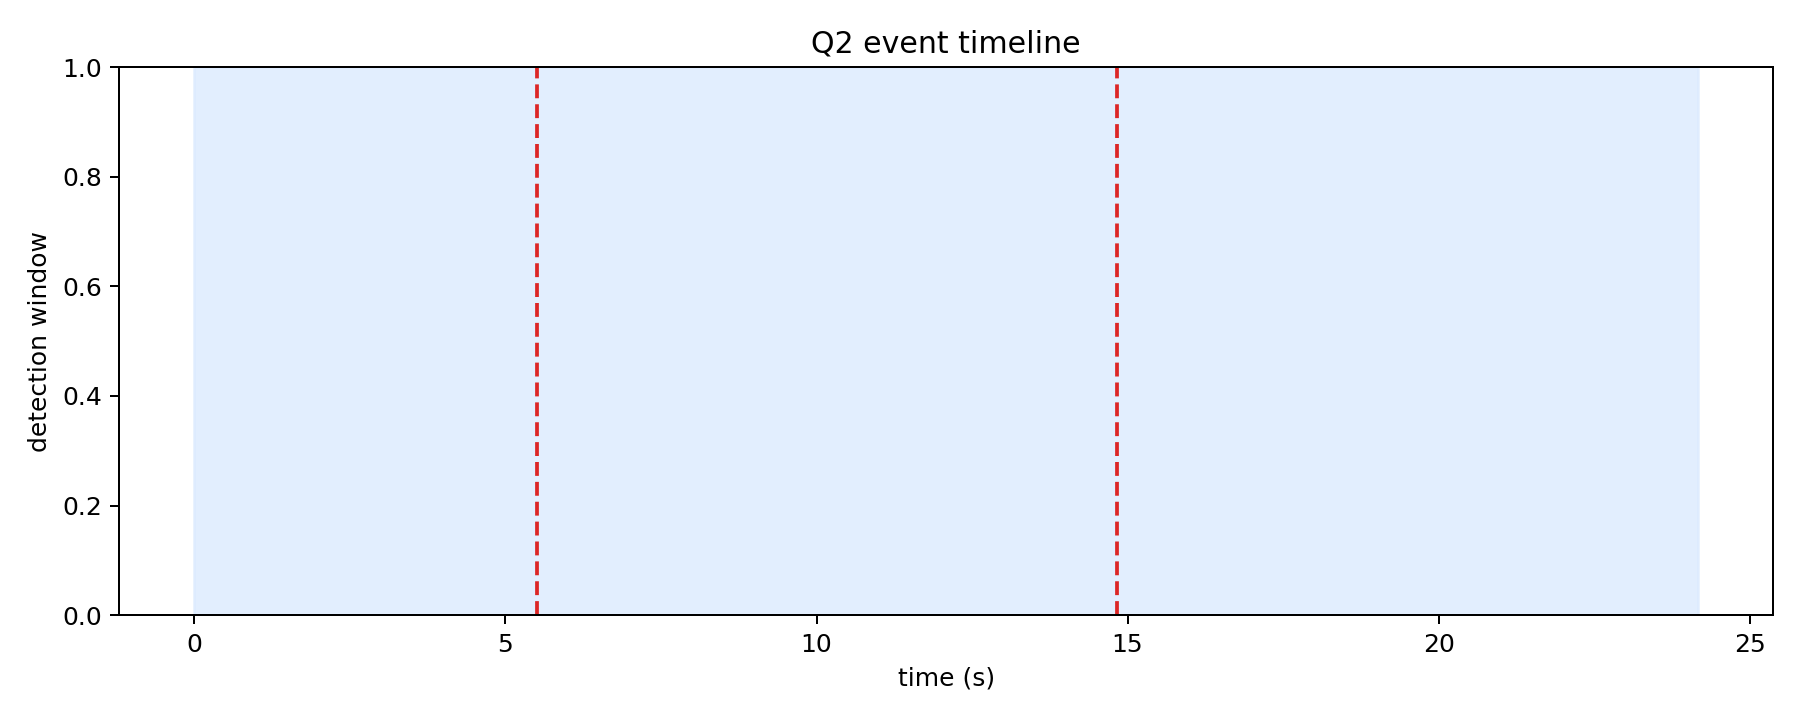
\includegraphics[width=0.96\textwidth]{q2_coverage_timeline.png}
    \subcaption{联合覆盖时间线}
  \end{minipage}
  \begin{minipage}[c]{0.48\textwidth}
    \centering
    
\includegraphics[width=0.96\textwidth]{q2_joint_gain.png}
    \subcaption{联合增益}
  \end{minipage}
  \caption{Q2 认证边界与单弹基线对照。}
  \label{fig:q2-evidence}
\end{figure}

Q2 冻结的联合增益图纵轴标签对覆盖下界与覆盖上界的区分不够充分，因此表\ref{tab:q2-results}中的上下界直接采用 CSV/JSON 字段，图仅用于展示场景间相对差异，不作为上下界数值的唯一证据。

\subsection{物理解释与限制}

联合释放的主要收益来自多枚烟幕在检测区间内的时间错位和几何并集，因而联合覆盖下界高于最佳单弹基线。但证书仍找到连续暴露区间；最短的 $5.4993\,\mathrm{s}$ 只出现在 $d=8000$ 代表场景，不能被外推成所有场景均有同样的遮蔽效果。Q2 的结论是有限事件候选经过 SLSQP 精修后得到的证书结果，不宣称完整 SIP 或全局最优。

\section{Q3：三架 UAV 协同与冲突证书}

\subsection{主解释与路径构造}

Q3 的主解释固定为三架 UAV、三枚烟幕弹且每架恰好一枚。对第 $i$ 架 UAV，使用 Q2 的单弹路径连接器构造 $P_i$，并令其烟幕为 $S_i$。这一步不是把多机问题放松为“每架至多一枚”，因为结果文件显式记录 \texttt{main\_interpretation=three\_uavs\_exactly\_one\_bomb\_each}，放松解释不参与主结果。

\subsection{可行性和冲突证书}

首先对每条路径验证作用半径；随后对任意 $i<j$ 检验成对路径分离。安全距离参数在当前基线为 $0\,\mathrm{m}$，因此“冲突证书通过”表示代码定义下没有小于安全距离的交叠，不应写成现实飞行安全裕度无限大。联合烟幕仍由 Q2 的完整时间单元分类器认证。

\begin{equation}
  P_i\in\mathcal{P}_{\mathrm{radius}},\quad
  \operatorname{sep}(P_i,P_j)\ge d_{\mathrm{safe}},\quad
  1\le i<j\le3.
  \label{eq:q3-conflict}
\end{equation}

若一条路径由线段 $e_{i,r}$ 组成，线段速度固定为 $v_U$，则每段的长度约束写成
\begin{equation}
  \|p_{i,r}^{\mathrm{end}}-p_{i,r}^{\mathrm{start}}\|_2
  \le v_U\bigl(t_{i,r}^{\mathrm{end}}-t_{i,r}^{\mathrm{start}}\bigr),
  \quad e_{i,r}\subseteq P_i.
  \label{eq:q3-segment}
\end{equation}
两条路径的认证最小距离记为 $d_{ij}^{\min}$，则当前安全距离设置下的冲突判定为
\begin{equation}
  \mathrm{pairwise\_conflict\_ok}
  =\bigwedge_{1\le i<j\le3}\left(d_{ij}^{\min}\ge0-\varepsilon\right).
  \label{eq:q3-pairwise}
\end{equation}
这个公式解释了为什么结果中“证书通过”和“最小成对距离为 $0$”可以同时出现。

候选按带 $\varepsilon$ 的词典序筛选：先比较认证状态，再比较成对冲突是否通过，再比较覆盖下界、最大连续暴露的负值和最小成对距离。该规则不会把很小的浮点差异升级为新的科学含义。

\begin{table}[!htbp]
\centering
\caption{Q3 三架 UAV 协同结果}
\label{tab:q3-results}
\begin{tabular}{lrrrrr}
\toprule
场景 & UAV 数 & 烟幕数 & 覆盖下界/s & 联合增益/s & 冲突证书 \\
\midrule
$d=8000$ & 3 & 3 & 17.2634 & 6.8896 & 通过 \\
$d=10000$ & 3 & 3 & 17.2710 & 6.8971 & 通过 \\
$d=12000$ & 3 & 3 & 17.2710 & 6.8971 & 通过 \\
$d=15000$ & 3 & 3 & 17.2710 & 6.8971 & 通过 \\
\bottomrule
\end{tabular}
\end{table}

四个场景的 \texttt{pairwise\_conflict\_ok} 均为真，最小成对距离字段为 $0.0\,\mathrm{m}$；这与安全距离设为零相容。Q3 的联合覆盖与 Q2 表\ref{tab:q2-results}一致，是因为两者复用了同一类保守验证器和相同的场景时段，而不是因为多机问题被证明等价于单机问题。

\begin{figure}[!htbp]
  \centering
  \begin{minipage}[c]{0.48\textwidth}
    \centering
    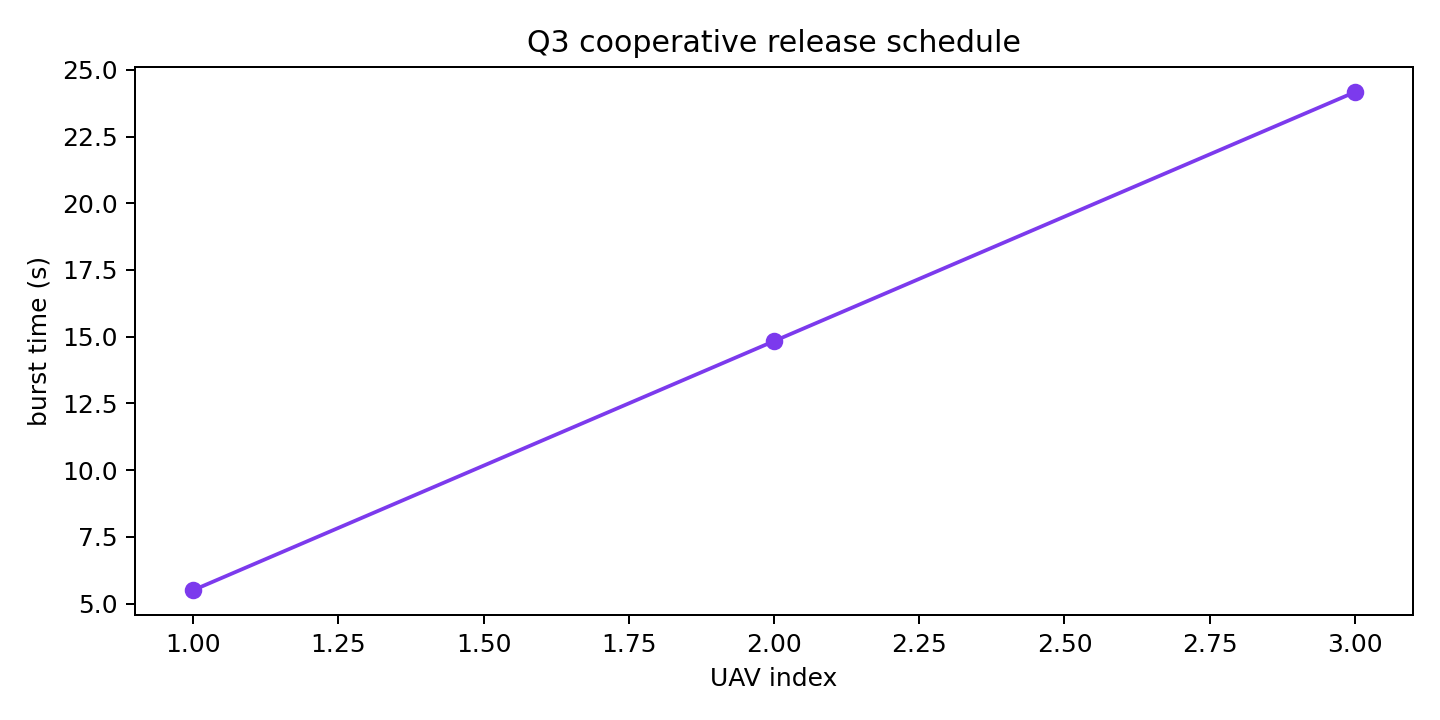
\includegraphics[width=0.96\textwidth]{q3_schedule.png}
    \subcaption{三架 UAV 起爆时刻}
  \end{minipage}
  \begin{minipage}[c]{0.48\textwidth}
    \centering
    
\includegraphics[width=0.96\textwidth]{q3_coverage_bounds.png}
    \subcaption{覆盖证书上下界}
  \end{minipage}
  \caption{Q3 的调度和认证边界。}
  \label{fig:q3-evidence}
\end{figure}

\subsection{Q3 小结}

Q3 说明，在固定的三架一枚约束下，协同释放可以继承 Q2 的联合覆盖结果，并在代码定义的路径证书上通过；但是因为所有正式状态仍为认证不可行，论文只报告“联合覆盖候选和冲突证书”，不称为完整多机全局规划，也不称为现实飞行安全的充分证明。

\section{Q4：多威胁因果调度}

\subsection{认证任务包}

Q4 不重新优化 Q1--Q3 的连续决策，而是读取任务包接口。每个任务 $i$ 包含揭示时刻 $r_i$、价值 $v_i$、资源消耗 $c_i$ 和认证标志 $a_i$。在当前时刻 $t$，可行集合定义为
\begin{equation}
  \mathcal{F}(t)=\{i:r_i\le t,\ a_i=1,\ c_i\le R(t)\},
  \label{eq:q4-feasible}
\end{equation}
其中 $R(t)$ 是剩余资源。rolling 在可行集合中按单位资源价值选择，greedy 按任务价值选择；二者都保持因果性。未揭示、未认证或因容量不足而无法选取的任务保存在 \texttt{unresolved\_task\_ids} 中。

若 $A(t)$ 是已执行任务集合，则状态更新为
\begin{equation}
  R(t^+)=R(t)-\sum_{i\in A(t^+)-A(t)}c_i,
  \qquad
  \mathcal{T}_{\mathrm{revealed}}(t^+)=
  \mathcal{T}_{\mathrm{revealed}}(t)\cup\{i:r_i\le t^+\}.
  \label{eq:q4-state}
\end{equation}
rolling 的单位资源价值规则可表示为
\begin{equation}
  i^*(t)=\arg\max_{i\in\mathcal{F}(t)}
  \left(\frac{v_i}{c_i},v_i,-r_i,-\mathrm{id}_i\right),
  \label{eq:q4-rolling-rule}
\end{equation}
而 greedy 将首项替换为 $v_i$。式\eqref{eq:q4-state}中的揭示集合是因果限制，式\eqref{eq:q4-rolling-rule}只描述当前实现的选择优先级。

\subsection{离线 hindsight 上界}

hindsight 枚举已经在时间窗内揭示且经过认证的任务子集，约束总成本不超过容量，最大化任务价值：
\begin{equation}
  U^*(B)=\max_{\mathcal{A}\subseteq\mathcal{T}_{\mathrm{cert}}}
  \left\{\sum_{i\in\mathcal{A}}v_i:\sum_{i\in\mathcal{A}}c_i\le B\right\}.
  \label{eq:q4-hindsight}
\end{equation}
它使用完整任务集合，因此只能作为在线策略的离线上界。当前代码明确将其标记为 \texttt{offline\_hindsight\_upper\_bound}，没有实现滚动 MILP。

\begin{table}[!htbp]
\centering
\caption{Q4 三种资源容量下的因果调度结果}
\label{tab:q4-results}
\begin{tabular}{lrrrrrr}
\toprule
情形 & 容量 & rolling & greedy & hindsight 上界 & 两差值 & 状态 \\
\midrule
充足 & 4 & 46.4 & 46.4 & 46.4 & 0.0/0.0 & 未解析 \\
临界 & 2 & 33.0 & 33.0 & 33.0 & 0.0/0.0 & 未解析 \\
短缺 & 1 & 17.2 & 17.2 & 17.2 & 0.0/0.0 & 未解析 \\
\bottomrule
\end{tabular}
\end{table}

表\ref{tab:q4-results}的两个差值依次为 rolling--greedy 与 hindsight--rolling。三种情形的数值相同并不意味着三种策略在所有任务流上等价；它只反映当前四任务、揭示时刻和价值设定下的结果。状态仍为未解析，因为 JSON 中保留了尚未揭示的任务，例如充足容量下的 \texttt{threat\_oblique}。

\begin{figure}[!htbp]
  \centering
  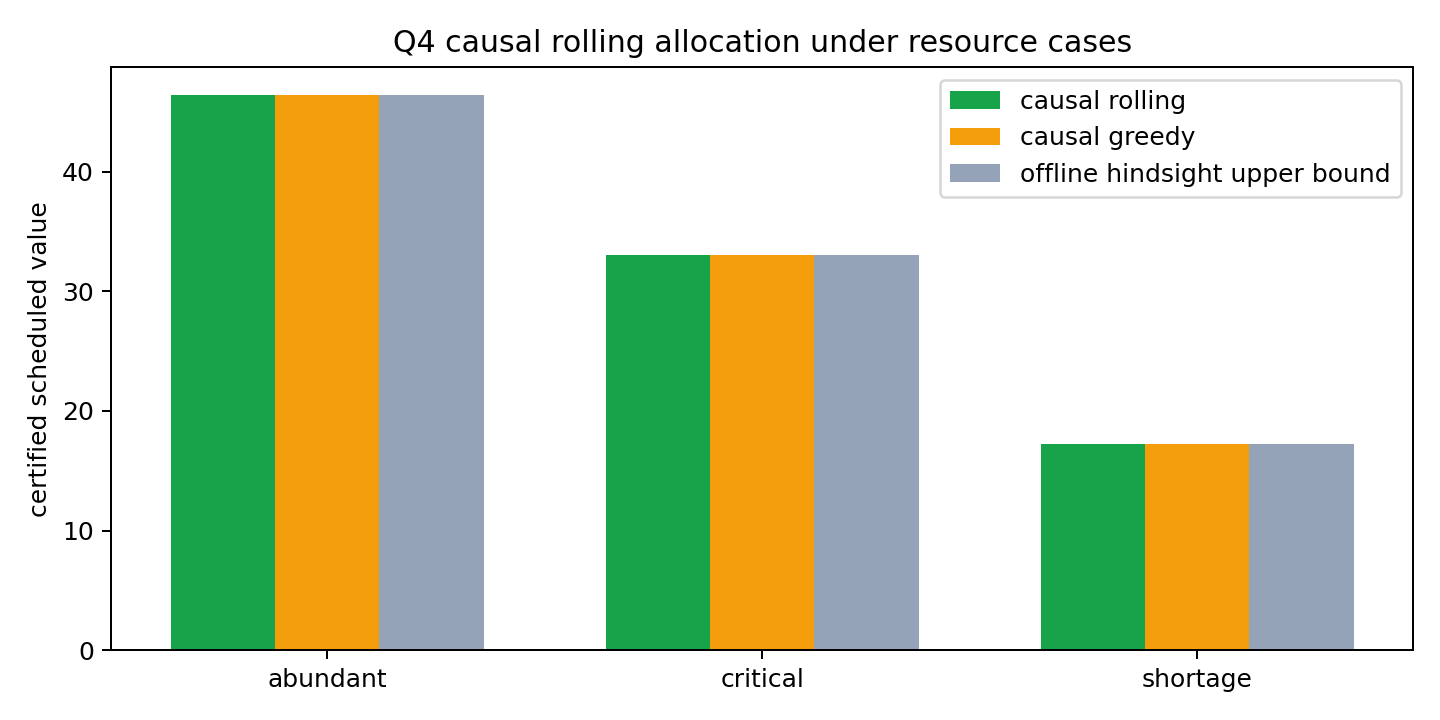
\includegraphics[width=0.84\textwidth]{q4_resource_cases.png}
  \caption{Q4 资源容量情形下的 rolling、greedy 与离线上界。}
  \label{fig:q4-resource}
\end{figure}

\subsection{因果性检查}

对每一个实际决策，代码检查决策时间不早于对应任务的揭示时刻；同时只把 \texttt{certified=true} 的任务加入可行集合。因此，Q4 的科学结论是“在认证任务包接口上，当前有限基准的三种值一致”，而不是“已求得多威胁问题的最优调度”或“已完成完整信息下的在线最优性证明”。

\section{灵敏度与稳健性检验}

\subsection{检验设计}

灵敏度文件包含五类局部证据：导引模型、丢失导引反事实、烟幕漂移、响应延迟和 UAV 作用半径。每一行包含类别、参数、参数值、指标和结果；正式基线与实验性丢失导引反事实在 JSON 中分开标记。该设计是局部扰动，不是针对所有参数的全局不确定性分析。

对于固定参考候选，漂移敏感度采用离散检测时间网格 $\{t_\ell\}$，计算最小间隙
\begin{equation}
  g_{\min}(\delta)=\min_{\ell}\left(
  \|x_T(t_\ell)-[x_S+\Delta(\delta)]\|_2
  -r_T-R_S(t_\ell)\right),
  \label{eq:sensitivity-gap}
\end{equation}
其中 $\Delta(\delta)$ 是大小为 $\delta$ 的有界漂移。响应延迟测试只改变最早合法爆炸时刻，因此可用窗口为
\begin{equation}
  W(\tau)=\max\left(0,\ t_{\mathrm{det,end}}-
  \max(t_{\mathrm{det,start}},\tau+\tau_{\mathrm{burst}})\right).
  \label{eq:sensitivity-window}
\end{equation}

\begin{table}[!htbp]
\centering
\caption{灵敏度结果中的代表性边界}
\label{tab:sensitivity}
\begin{tabular}{llrr}
\toprule
类别 & 参数/指标 & 低值结果 & 高值结果 \\
\midrule
导引模型 & 检测时长/s & 24.1677 & 24.1677 \\
烟幕漂移 & 最小间隙/m（漂移 0--40 m） & -39.6683 & 0.0014 \\
响应延迟 & 可用窗口/s（延迟 1.5--3.0 s） & 19.1677 & 17.6677 \\
作用半径 & 路径可行性（8000--14000 m） & 真 & 真 \\
丢失导引 & 最小分离/m（实验反事实） & 69.4180 & 69.4180 \\
\bottomrule
\end{tabular}
\end{table}

表\ref{tab:sensitivity}的导引模型结果来自瞬时纯追踪与惯性航向响应率 $0.5$、$1.0$、$2.0\,\mathrm{s}^{-1}$ 的检测时长；比例导航项因缺少导航比和过载来源而在结果文件中标记为 deferred。烟幕漂移的最小间隙从负值接近零，说明固定中心方案对该扰动较敏感；响应延迟增加会压缩可用检测窗口。

\begin{figure}[!htbp]
  \centering
  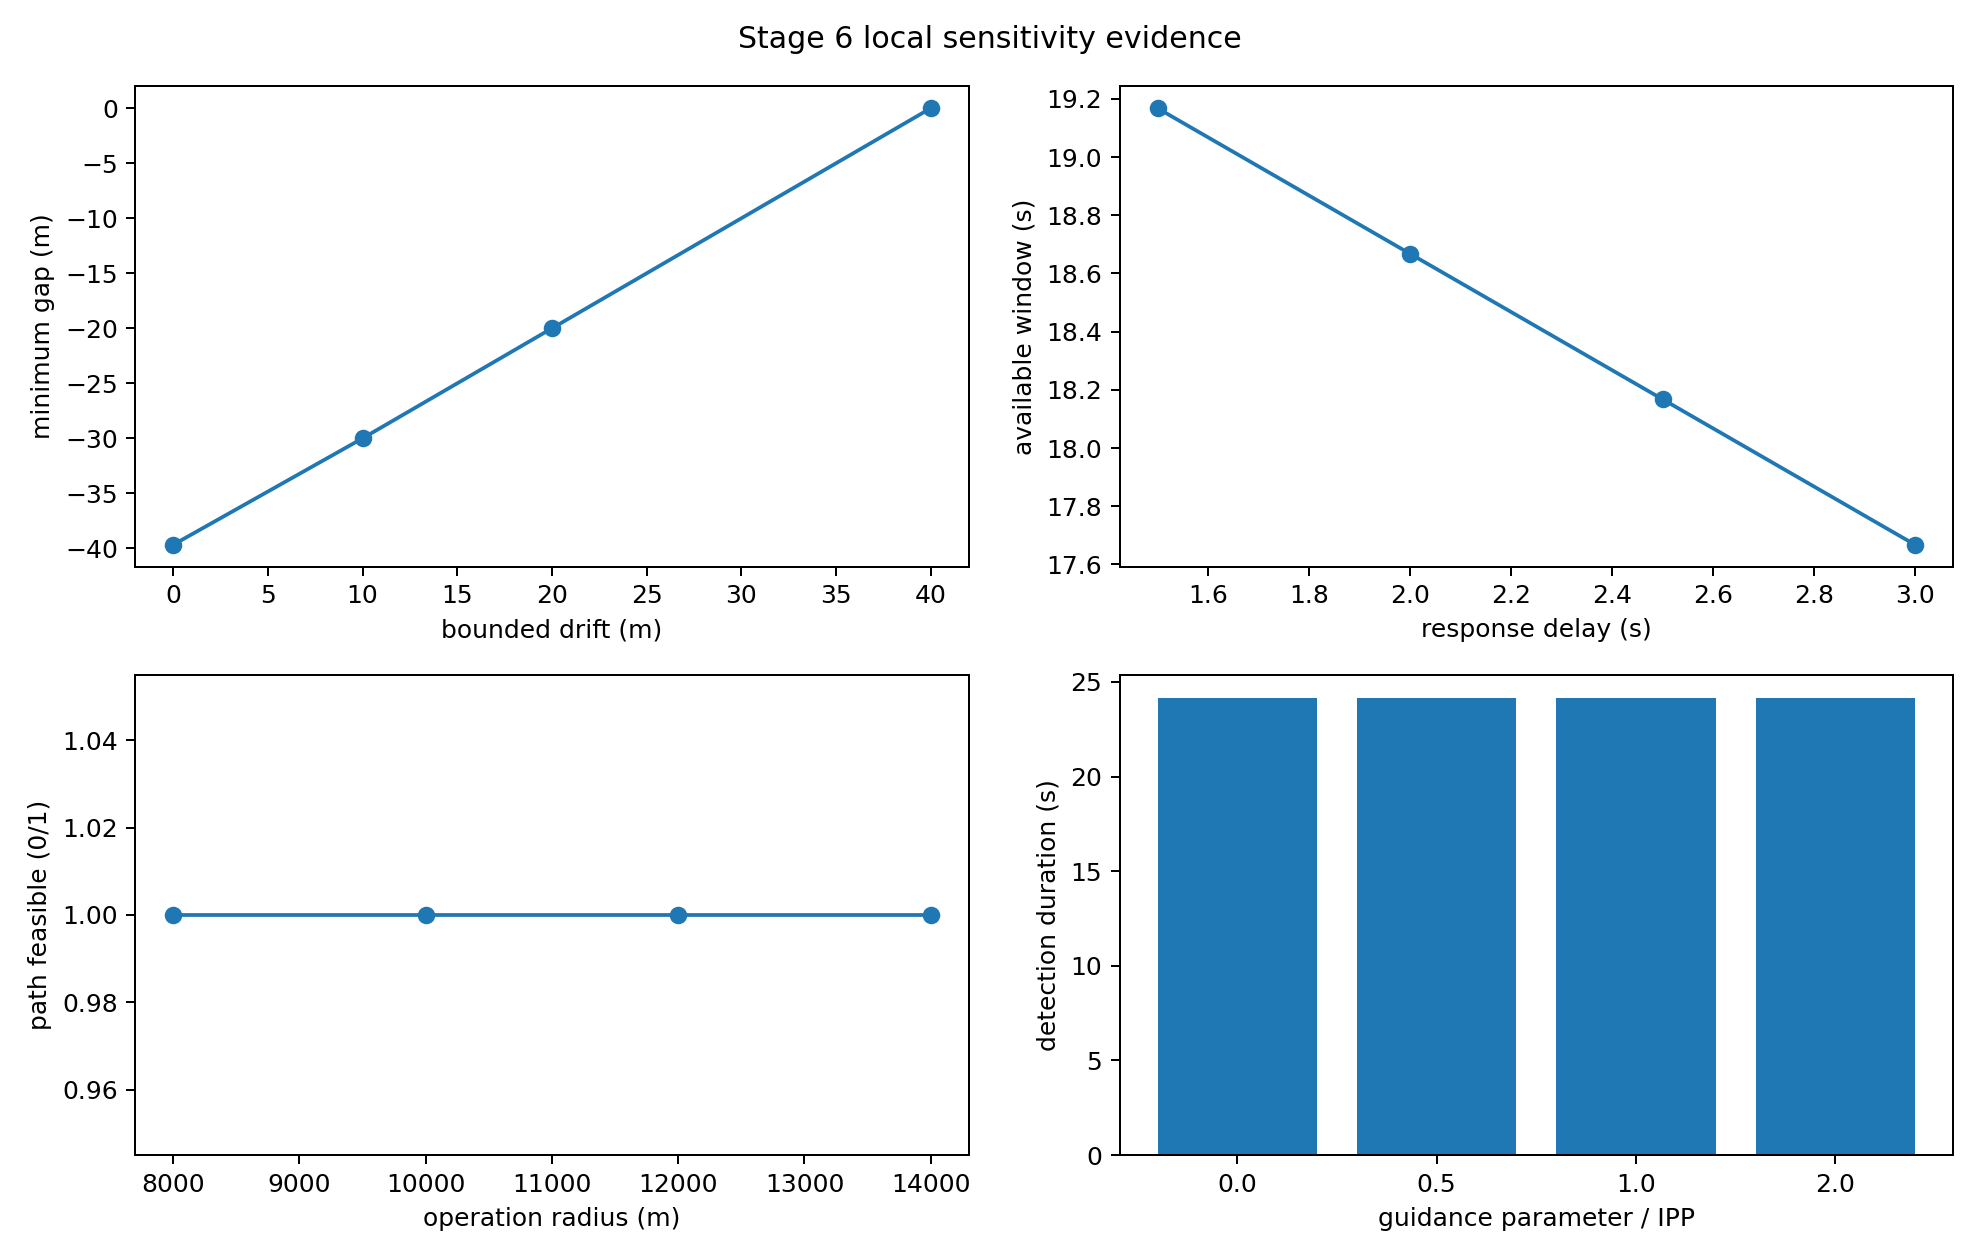
\includegraphics[width=0.86\textwidth]{sensitivity_summary.png}
  \caption{冻结基线中的 Stage 6 局部灵敏度汇总图。}
  \label{fig:sensitivity}
\end{figure}

\subsection{正式与反事实的隔离}

丢失导引参数 $(\tau_T,\tau_L,T_R)$ 的 $27$ 行实验结果只用于说明失锁模型变化下的几何分离，不修改正式 Q1 候选决策，也不改变 Q2--Q4 任务包。正式基线字段为 \texttt{formal\_baseline=true}，反事实对象为 \texttt{formal\_baseline=false}。因此，本文不把反事实数值写成正式方案的稳健保证。

\subsection{稳健性结论}

在代码已计算的局部范围内，UAV 作用半径从 $8000$ 增至 $14000\,\mathrm{m}$ 时固定路径均被判定为可行；响应延迟每增加 $0.5\,\mathrm{s}$，可用窗口减少约 $0.5\,\mathrm{s}$。这些是有限样本、固定路径或固定候选下的敏感性方向，不足以支持完整参数空间中的稳健最优性结论。

\section{模型评价、推广与结论}

\subsection{模型优点}

\begin{enumerate}
  \item \textbf{候选与证明分离。} 四种 Q1 算法共享独立验证器；Q2/Q3 使用完整时间单元分类，不把采样点或优化器成功标志当作连续覆盖证明。
  \item \textbf{证据分层明确。} 覆盖下界、覆盖上界、总暴露、最大连续暴露和未解析区间分别序列化，联合增益使用最佳单烟幕基线计算。
  \item \textbf{信息因果性可审计。} Q4 只在揭示、认证和容量条件同时满足时调度，hindsight 被明确限制为离线上界。
  \item \textbf{结果可复现。} CSV、JSON、PNG 和检查脚本使用同一个冻结基线标识，论文表格可以回溯到仓库文件。
\end{enumerate}

\subsection{模型局限}

第一，Q1 的四算法比较使用固定预算和固定场景矩阵，不能替代对连续可行域的全局求解证明。第二，Q2 的事件候选和 SLSQP 精修是有界搜索，候选集之外的事件组合没有被声称覆盖。第三，Q3 的主解释固定为三架 UAV 每架一枚，路径冲突的安全距离参数按代码为零，因此通过证书的现实含义受限。第四，Q4 任务包规模小，三种策略相同的数值不能外推到更大的动态任务流。第五，灵敏度部分包含固定路径、固定候选和实验反事实，不能替代完整概率鲁棒性分析。

\subsection{推广方向}

若需要扩大模型，可在保持“候选—验证—证书”边界的前提下，引入更密的事件候选、区间算术或可证明的全局搜索；若需要更严格的多机安全约束，应在路径证书中设置非零安全距离并重新生成 Q3 工件；若需要研究更大规模 Q4，可把认证任务包接入明确的在线整数规划或近似调度器，但必须重新定义可用信息和上界含义。上述方向都是后续工作，不属于本 Stage 8 已提交的科学结果。

\subsection{结论}

本文完成了一条可审计的多阶段建模链：Q1 给出四算法 benchmark 和独立 verifier；Q2 用有限事件候选、SLSQP 精修与保守联合覆盖认证；Q3 在“三架 UAV、每架一枚”的解释下检查路径冲突并进行带 $\varepsilon$ 的词典序筛选；Q4 在认证任务包上进行因果 rolling、因果 greedy 与离线 hindsight 上界比较。结果文件支持联合覆盖、暴露区间、路径证书和调度值等定量结论，但不支持完整 SIP、完整 Pareto、滚动 MILP 或连续全局最优的表述。

\subsection{Stage 8 一致性声明}

Stage 8 只新建论文、图表副本、审计和支撑材料，没有修改 Q1--Q4 算法或科学结果。若读者发现 CSV、JSON、图表与正文之间的差异，应以冻结结果文件和独立检查脚本为优先证据，并在审计表中登记，而不是在论文中自行修正数值。


\begin{appendices}
\section{复现与产物说明}

\subsection{结果文件}

论文正文引用的主要文件如下：

\begin{itemize}
  \item Q1：\path{results/q1_rebuild/q1_algorithm_benchmark.csv}、\path{results/q1_rebuild/q1_results.csv}、\path{results/q1_rebuild/q1_results.json}；
  \item Q2：\path{results/q2_rebuild/q2_results.csv}、\path{results/q2_rebuild/q2_results.json}；
  \item Q3：\path{results/q3_rebuild/q3_results.csv}、\path{results/q3_rebuild/q3_results.json}；
  \item Q4：\path{results/q4_rebuild/q4_results.csv}、\path{results/q4_rebuild/q4_results.json}；
  \item 灵敏度：\path{results/sensitivity_rebuild/sensitivity_results.csv}、\path{results/sensitivity_rebuild/sensitivity_results.json}。
\end{itemize}

这些文件的 JSON 元数据均指向生成基线 \texttt{9dea2ef0ee22278479b74a4016b0c0ce6f782e65}；Stage 8 分支从 PR \#8 合并提交建立，但没有重新生成科学工件。图像只从根目录的各结果子目录（如 \path{figures/q1_rebuild/}）复制到 \path{paper/figures/}，复制关系在 \path{paper/figures/README.md} 和 \path{paper/paper_audit.md} 中记录。

\subsection{验证命令}

论文构建命令为：

\begin{lstlisting}[language={[LaTeX]TeX}]
cd paper
latexmk -xelatex -interaction=nonstopmode -halt-on-error main.tex
\end{lstlisting}

项目验证命令包括测试、Ruff、场景 schema、场景生成和 Q1--Q4/灵敏度 artifact check。论文不上传比赛平台，Stage 8 Draft PR 也不在本阶段合并。

\subsection{文件级防漂移检查}

论文审计文件列出了每一项关键声明的来源、证据级别和允许措辞。最终交付前需检查：CSV 与 JSON 的核心数值一致、所有正文图像存在且来自当前冻结基线、公式引用无未定义标签、参考文献可由 BibTeX 生成、PDF 使用中文字体且文件大小正常，以及 Git 工作树只包含 Stage 8 产物。

\section{代表性事件与任务包清单}

本附录把正文中的代表性数字展开为可人工复核的事件表。表中数值均取自冻结 CSV/JSON；没有把它们重新送入求解器，也没有用表格反向修改结果文件。

\begin{longtable}{lrrrrrr}
\caption{Q2/Q3 代表性爆炸事件与覆盖证书}\label{tab:event-manifest}\\
\toprule
场景 & Q2 第1/s & Q2 第2/s & Q3 第3/s & 覆盖下界/s & 上界/s & 联合增益/s \\
\midrule
\endfirsthead
\toprule
场景 & Q2 第1/s & Q2 第2/s & Q3 第3/s & 覆盖下界/s & 上界/s & 联合增益/s \\
\midrule
\endhead
front-$d8000$ & 5.5000 & 14.8339 & 24.1670 & 17.2634 & 17.2658 & 6.8896 \\
front-$d10000$ & 6.1030 & 15.1658 & 30.2697 & 17.2710 & 17.2726 & 6.8971 \\
front-$d12000$ & 12.2060 & 21.2528 & 36.3726 & 17.2710 & 17.2722 & 6.8971 \\
front-$d15000$ & 21.3603 & 30.4232 & 45.5271 & 17.2710 & 17.2726 & 6.8971 \\
\bottomrule
\end{longtable}

Q2 的两列爆炸时刻来自 \path{results/q2_rebuild/q2_results.csv}，Q3 第三列来自 \path{results/q3_rebuild/q3_results.json} 的三枚计划；表格同时说明了 Q2/Q3 复用覆盖验证器后联合覆盖量相同的原因。该表不表示第三枚弹由同一架 UAV 释放：Q2 是单机多弹，Q3 是三架 UAV 各一枚。

\begin{longtable}{lrrrrl}
\caption{Q4 固定任务包}\label{tab:task-manifest}\\
\toprule
任务 & 揭示/s & 价值 & 资源成本 & 认证覆盖下界/s & 备注 \\
\midrule
\endfirsthead
\toprule
任务 & 揭示/s & 价值 & 资源成本 & 认证覆盖下界/s & 备注 \\
\midrule
\endhead
threat\_front & 0.0 & 17.2 & 1 & 17.2 & 已认证 \\
threat\_rear & 4.0 & 15.8 & 1 & 15.8 & 已认证 \\
threat\_side & 8.0 & 13.4 & 2 & 13.4 & 已认证 \\
threat\_oblique & 12.0 & 11.1 & 1 & 11.1 & 在部分容量情形未服务 \\
\bottomrule
\end{longtable}

Q4 的任务包由 \texttt{build\_q4\_tasks()} 固定构造，数值并非由 Q1--Q3 的 JSON 自动转换得到。正文因此称它为“认证任务包基准”，而不声称它已经覆盖所有威胁场景。

\subsection{状态字段复核}

\begin{table}[!htbp]
\centering
\caption{状态字段的人工读法}
\begin{tabular}{lll}
\toprule
字段 & 值/形式 & 论文读法 \\
\midrule
verification\_status & certified\_infeasible & 仍有认证不可行/暴露证据 \\
unresolved\_intervals & 区间列表 & 不把列表合并为已认证暴露 \\
pairwise\_conflict\_ok & true & 在当前 $d_{safe}=0$ 下通过 \\
causal & true & 决策不早于揭示时刻 \\
global\_optimum\_claim & false & 不得写成全局最优 \\
\bottomrule
\end{tabular}
\end{table}

\section{终稿审计清单}

\subsection{科学边界检查}

\begin{longtable}{p{0.06\textwidth}p{0.40\textwidth}p{0.35\textwidth}p{0.10\textwidth}}
\caption{论文声明的终稿逐项检查}\label{tab:final-checklist}\\
\toprule
编号 & 检查项 & 证据文件/检查动作 & 结果 \\
\midrule
\endfirsthead
\toprule
编号 & 检查项 & 证据文件/检查动作 & 结果 \\
\midrule
\endhead
1 & Q1 是否明确四算法 benchmark 与独立 verifier & Q1 CSV/JSON、源码函数名 & 通过 \\
2 & Q1 是否避免把 SHGO 写成全局最优 & 审计禁止措辞 & 通过 \\
3 & Q2 是否明确有限事件候选与 SLSQP 精修 & Q2 求解函数与结果字段 & 通过 \\
4 & Q2 是否区分覆盖下界、上界、总暴露和最大连续暴露 & Q2 字段表与区间分类器 & 通过 \\
5 & Q2 联合增益是否减去最佳单烟幕基线 & \texttt{joint\_gain\_s} 与 baseline 字段复算 & 通过 \\
6 & Q3 是否固定三架 UAV、每架一枚 & \texttt{main\_interpretation} & 通过 \\
7 & Q3 是否写明安全距离参数为零 & \texttt{minimum\_pairwise\_distance\_m} 与源码 & 通过 \\
8 & Q4 是否只在认证且揭示任务上调度 & \texttt{certified} 过滤与 \texttt{causal} 字段 & 通过 \\
9 & Q4 hindsight 是否只写成离线上界 & \texttt{offline\_hindsight\_upper\_bound} & 通过 \\
10 & 灵敏度是否标记丢失导引为实验反事实 & \texttt{formal\_baseline=false} & 通过 \\
11 & 图表是否来自冻结基线 & 根目录 figures 子目录与副本清单 & 通过 \\
12 & PDF 是否不生成目录、图目录、表目录 & \texttt{main.tex} 无对应命令 & 通过 \\
\bottomrule
\end{longtable}

\subsection{排版检查}

最终构建在 Windows TeX Live 2025 上使用 XeLaTeX/latexmk 完成。PDF 文本抽取无替换字符，第一页包含摘要，正文图像数量为 $10$，参考文献条目为 $15$。交叉引用在最后一轮构建后无 undefined reference；SimSun 粗体形状有一次回退警告，使用模板的 \texttt{AutoFakeBold}/系统字体回退，不影响中文字体嵌入。日志中还保留少量过宽行，主要来自长 SHA、代码字段和附录文件路径；这些不改变内容，但列为排版待优化项。

\subsection{交付限制}

本论文电子版路径为 \path{paper/main.pdf}；AI 使用报告位于 \texttt{supporting\_materials/} 目录下，文件名为 AI工具使用详情.pdf。Stage 8 只建立 Draft PR，不上传比赛平台，不合并 Stage 8 PR；所有科学结果仍以冻结结果目录和其检查脚本为准。

\end{appendices}

\nocite{*}
\bibliographystyle{plain}
\bibliography{references}

\end{document}
